\chapter{Einleitung}\label{sec:exp_einleitung}

Die \gls{ibv} ist ein essenzieller Bestandteil moderner Fertigungsprozesse und Qualitätskontrollsysteme. Als Teilgebiet des maschinellen Sehens, auch bekannt als \gls{cv}, ermöglicht sie Maschinen und Systemen, visuelle Informationen aus Produktionsprozessen und Produkten zu erfassen und zu analysieren. Dadurch können Aufgaben wie \textbf{Qualitätskontrolle}, \textbf{Inspektion}, \textbf{Positionierung} und \textbf{Vermessung} automatisiert durchgeführt werden, was zur Steigerung der Produktqualität und Effizienz der Prozesse und Kostensenkung beiträgt \citep{cognex_grundlagen_nodate}.

Nach \citep{jahne_digitale_2024} ist unter \gls{cv} ein Computersystem zu verstehen, das die gleiche Aufgabe wie ein biologisches System erfüllt, nämlich aus Bildern zu erkennen, was in der Welt ist und wo es sich befindet. Während Menschen aufgrund evolutionärer Entwicklungen visuelle Informationen intuitiv verarbeiten, haben \gls{cv}-Algorithmen nach wie vor Schwierigkeiten, dieselben Aufgaben zuverlässig zu bewältigen \citep[S.~3]{szeliski_computer_2022}. 

In den letzten Jahren allerdings hat die Komplexität industrieller Problemstellungen stark zugenommen, sodass traditionelle Methoden der Bildverarbeitung oft nicht mehr ausreichen \citep[S.~442]{suse_bildverarbeitung_2014}. \gls{knn} übertreffen mittlerweile bei idealen Bilddaten sogar die menschliche Wahrnehmung \citep{dodge_study_2017}. Durch den Einsatz von \gls{dl}-Methoden können komplexe und variierende Prüfaufgaben wie \textbf{Objektdetektion}, \textbf{Bildklassifikation} und \textbf{Segmentierung} effizient automatisiert werden \citep{kaur_systematic_2024, manakitsa_review_2024}.

Der Einsatz von \gls{dl} führt aber auch zu Veränderungen im Gesamtprozess. Neue Teilprozesse wie das Training von \gls{knn} sind bereits hinreichend wissenschaftlich untersucht. Insbesondere erfordern diese Modelle große Mengen an Trainingsdaten, um zuverlässig zu funktionieren, und sind empfindlich gegenüber Bildrauschen und anderen Störfaktoren \citep{dodge_study_2017}. In industriellen Anwendungen stehen jedoch oft nur begrenzte Datenmengen zur Verfügung, und die Bilddaten können aufgrund von Produktionsbedingungen Rauschen oder Qualitätsmängel aufweisen.

\textbf{Ziel dieser Arbeit} ist es daher, die Entwicklung und Evaluierung einer \gls{dl}-Anwendung vorzustellen, die spezifische Merkmale in industriellen Bildern automatisch erkennen und segmentieren kann. Insbesondere wird die UNet-Architektur betrachtet, die sich in ähnlichen Anwendungsfällen bewährt hat.

\section{Motivation}\label{expose_motivation}

Im Rahmen meines Praxissemesters bei der Gefasoft GmbH in Regensburg hatte ich die Gelegenheit, mich intensiv mit unterschiedlichen Projekten der \gls{ibv} zu befassen. Im Bildverarbeitungs-Labor konnte ich einen tiefen Einblick in die vielfältigen Projekte der Sichtprüfung gewinnen. Zu den typischen Aufgaben in diesem Bereich zählen unter anderem die Objekterkennung, Oberflächeninspektion und Vollständigkeitsprüfung \cite[S. 5]{demant_industrielle_2011}.

Die Umsetzung der genannten Prozesse umfasst eine Reihe von Schritten, die von der Bildaufnahme und -vorverarbeitung bis zur Analyse und Bewertung der Bilddaten reichen (s. Abbildung \ref{fig:vorgehensmodell}). Im Rahmen dessen werden spezifische Vorgaben und Ziele definiert, um die gewünschten Informationen aus einem Bild zu extrahieren und in der realen Welt existierende Objekte zu erfassen. Im Anschluss erfolgt die Separierung der Objekte vom Hintergrund. Diesbezüglich werden Regionen konstanter Merkmale und Diskontinuitäten durch eine Segmentierung identifiziert \cite[S.13]{jahne_digitale_2024}.

\begin{figure}[h]
    \centering
    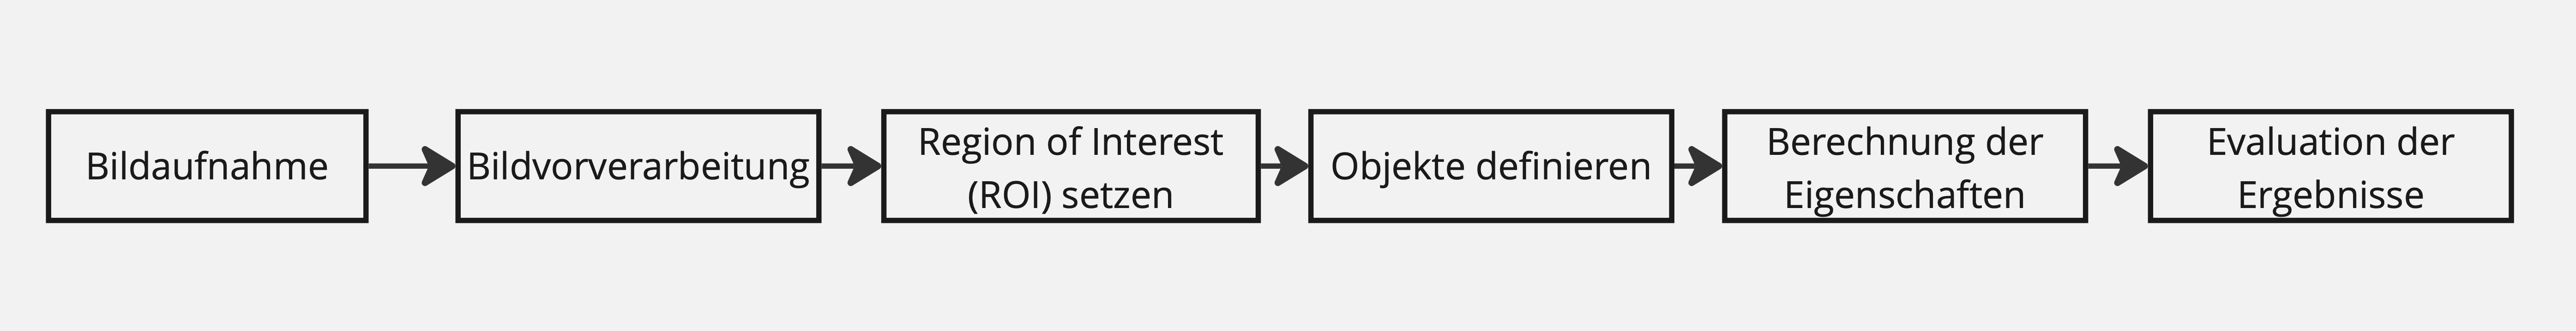
\includegraphics[width=1\linewidth]{expose/Vorgehensmodell_IBV.jpg}
    \caption{Vorgehensmodell der industriellen Sichtprüfung laut \cite[S.15]{demant_industrielle_2011}}
    \label{fig:vorgehensmodell}
\end{figure}

Für eine exakte Objekterkennung ist es in vielen Fällen erforderlich, die genannten Schritte mehrfach zu durchlaufen und \textbf{die Parameter}(besser die Parameter erklären) anzupassen. Dies stellt jedoch lediglich eine einfache Aufgabe dar, sofern sich ein Objekt klar vom Hintergrund unterscheidet. Eigenschaften wie spezielle Texturen, Formen, Farben oder Größen von Objekten können die zuverlässige Detektion erschweren, da Fehler mit dem Hintergrund verschmelzen und somit eine präzise Analyse verhindern. Dies wird durch die Beispiele in Abbildung \ref{fig:image2} verdeutlicht, die Fälle darstellen, die in der Praxis nicht mit traditionellen Algorithmen gelöst werden können.

\begin{figure}[h]

\begin{subfigure}{0.5\textwidth}
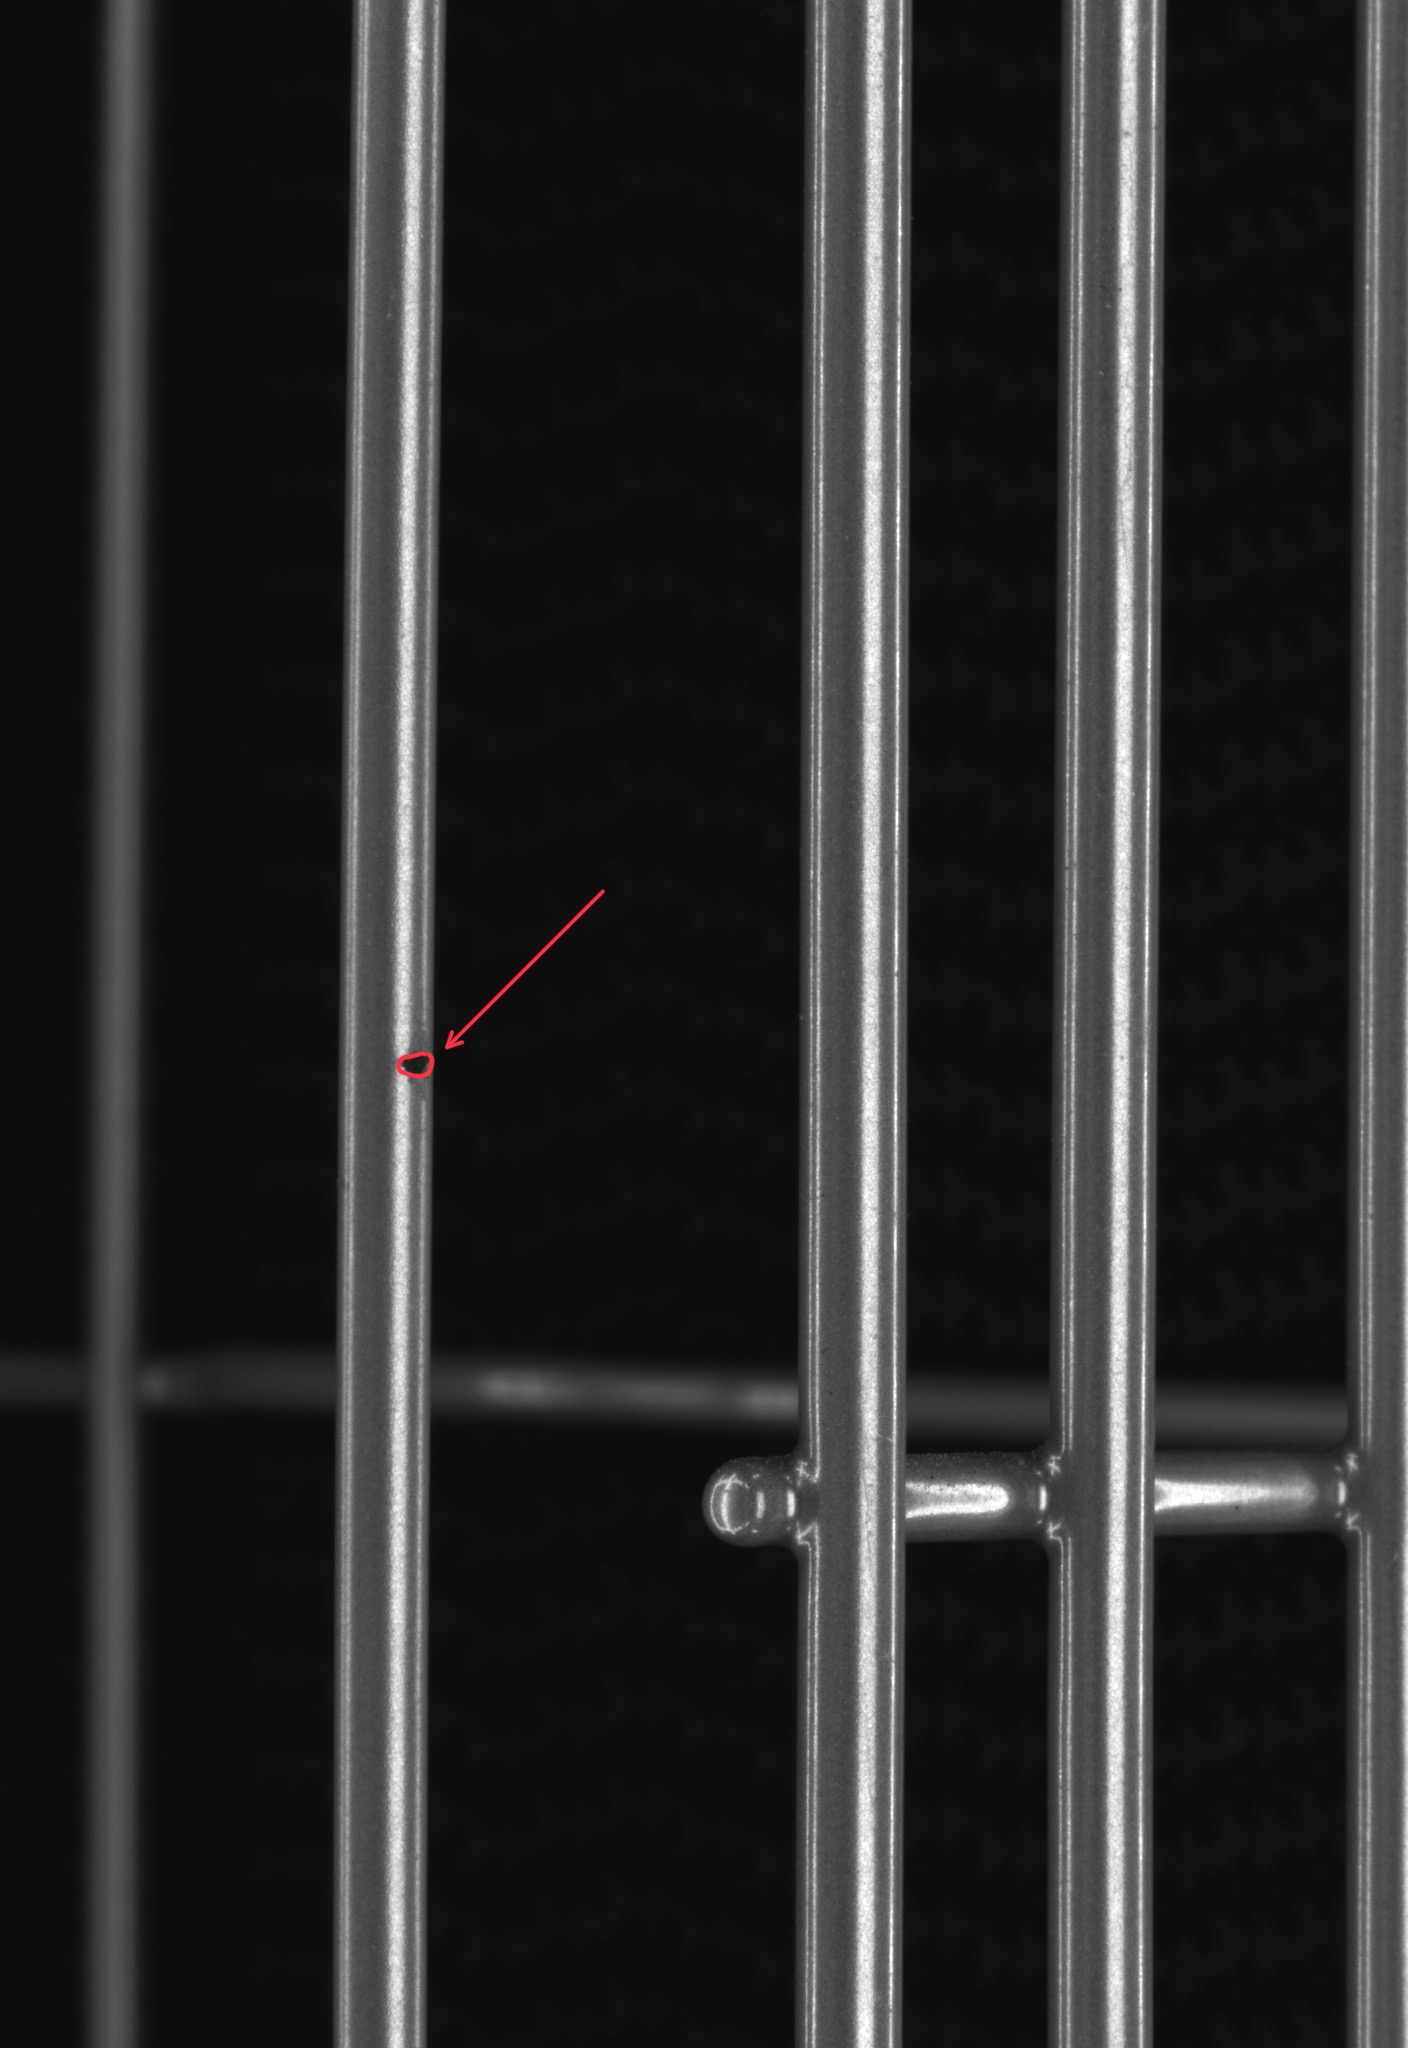
\includegraphics[width=0.9\linewidth, height=6cm]{expose/Fehler.jpg} 
\caption{Verschmutzung an einem Draht; das gesuchte Merkmal ist aufgrund seiner geringen Größe kaum zu erkennen. Die Verschmutzungen haben denselben Grauwert wie der Hintergrund.}
\label{fig:subim1}
\end{subfigure}
\begin{subfigure}{0.5\textwidth}
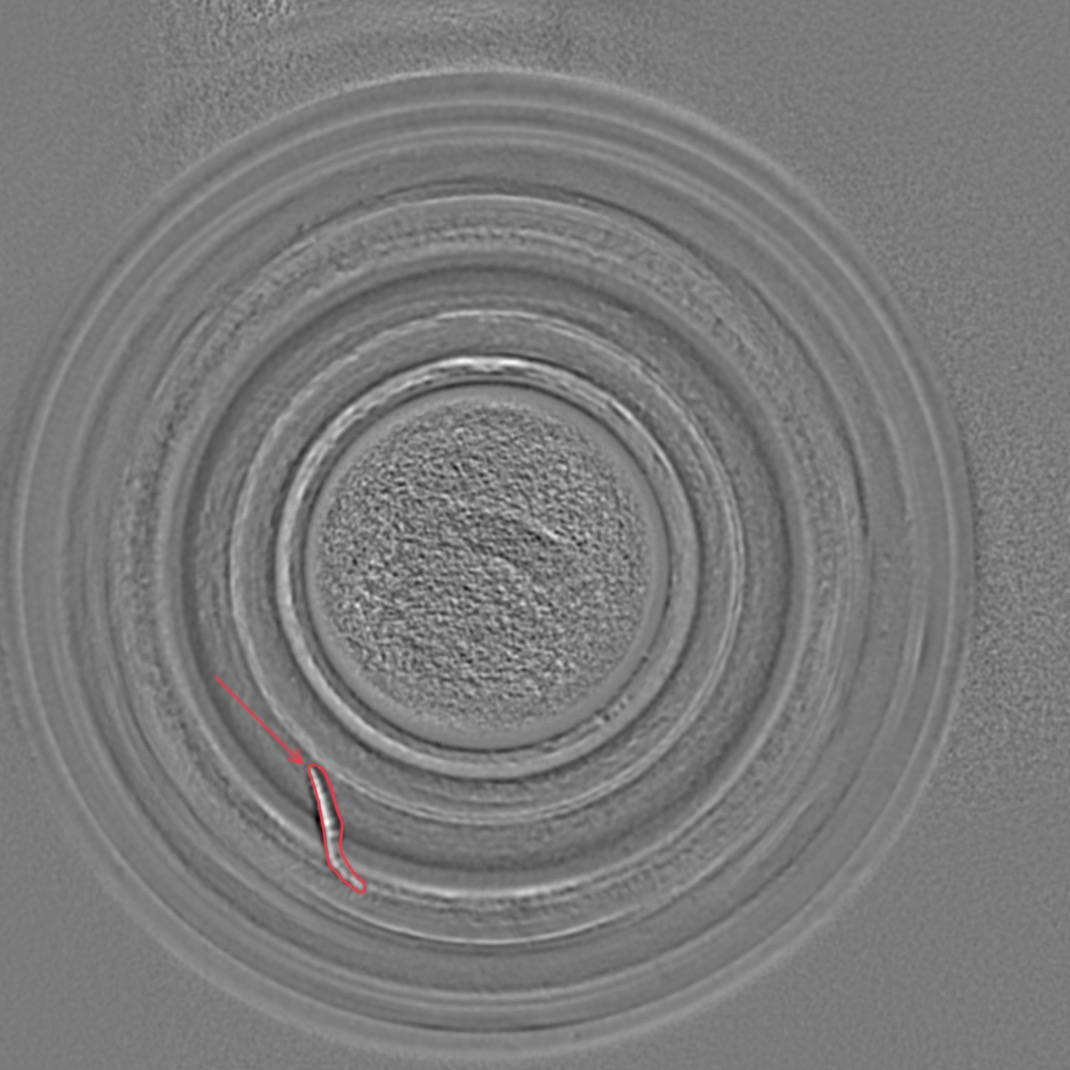
\includegraphics[width=0.9\linewidth, height=6cm]{expose/Kratzer.jpg}
\caption{Kratzer an einem Musterteil; die Fehler weisen sehr ähnliche Muster wie die fehlerfreien Abschnitte des Musterteils auf. Die Graustufen des gesuchten Merkmals ähneln stark denen des Bildhintergrunds.}
\label{fig:subim2}
\end{subfigure}

\caption{Beispiele aus der Praxis der Sichtprüfung. Die Bilder wurden bereits mittels Bildvorverarbeitungsalgorithmen verbessert, um eine höhere Bildqualität zu erzielen. Die gesuchten Merkmale wurden händisch gekennzeichnet, um dem Leser einen Überblick zu verschaffen.}

\label{fig:image2}
\end{figure}

Durch die tiefen Schichten neuronaler Netze können komplexe Merkmalsrepräsentationen gelernt werden, die feinere Details und abstrakte Muster erkennen lassen. Beispielsweise haben \gls{cnn} in der Oberflächeninspektion hohe Genauigkeiten bei der Erkennung von Defekten auf Metalloberflächen erreicht \citep{saberironaghi_defect_2023}.

Angesichts dieser Fortschritte möchte ich in meiner Arbeit untersuchen, wie \gls{dl}-Methoden. Ziel ist es zu demonstrieren, dass mithilfe dieser Methoden auch in anspruchsvollen Szenarien eine präzise Objekterkennung und Segmentierung möglich ist, in denen traditionelle Methoden versagen.

\section{Problemstellung}\label{expose_problemstellung}

Ein Beispiel für den Einsatz von \gls{dl}-Modellen in der \gls{ibv} ist ShuffleDefectNet, das auf dem NEU-Datensatz eine Genauigkeit von 99,75 \% erreichte \cite{saberironaghi_defect_2023}. Dieses Modell erfordert eine große Anzahl von fehlerfreien und fehlerhaften Beispielen in den Trainingsdaten. Es wird mit korrekt gelabelten Daten trainiert, um zwischen fehlerfreien und fehlerhaften Mustern zu unterscheiden. Der NEU-Datensatz umfasst insgesamt 1.800 Bilder, die in sechs verschiedene Defektklassen mit jeweils 300 Bildern unterteilt sind.

Im Gegensatz dazu sind Bildverarbeitungsaufgaben aus der Praxis meist auf spezifische Produkte, Materialien oder Defekte fokussiert. Ein industrieller Datensatz könnte beispielsweise ausschließlich Bilder eines speziellen Musterteils mit bestimmten Arten von Kratzern oder Defekten enthalten. Da es für verschiedene Anwendungsfälle keine öffentlich zugänglichen Datensätze gibt, entstehen häufig relativ kleine Datensätze, deren zu detektierende Merkmale oder Regionen in den Bildern manuell annotiert werden müssen.

Zusammenfassend besteht die Problemstellung darin:

\begin{itemize} 
\item \textbf{Spezialisierte Aufgabenstellung}: Das Modell soll spezifische Merkmale oder Anomalien erkennen, die nur in diesem speziellen Kontext relevant sind. 
\item \textbf{Begrenzte Datenmenge}: Aufgrund der Spezialisierung ist die Anzahl der verfügbaren Trainingsdaten oft gering. Es ist aufwändig und kostspielig, große Mengen an industriellen Bilddaten zu sammeln und zu annotieren, insbesondere wenn es um seltene Defekte oder spezifische Produktionsbedingungen geht. 
\end{itemize}

Künstliche neuronale Netze (\gls{knn}) erfordern in der Regel große Datenmengen, wenn sie mittels überwachtem Lernen trainiert werden, um eine gute Generalisierungsfähigkeit zu entwickeln und somit zuverlässige Ergebnisse zu liefern \cite{lecun_deep_2015}.

Im Rahmen dieser Arbeit sind die Fortschritte im medizinischen Bereich von besonderem Interesse, da die dortigen Herausforderungen denen unseres Datensatzes ähneln. Ein Beispiel dafür ist das U-Net-Modell von Ronneberger et al. (2015) \cite{ronneberger_u-net_2015}, das speziell für die effiziente Segmentierung komplexer Mikroskopiebilder in der Biomedizin entwickelt wurde.

Das U-Net-Modell kann mit sehr wenigen Bildern trainiert werden und zeigt dennoch eine überlegene Leistung bei Aufgaben der biomedizinischen Bildsegmentierung. Es nutzt intensiv Datenaugmentation, um die begrenzte Anzahl annotierter Beispiele effizient zu nutzen.

In den letzten Jahren wurde die U-Net-Architektur erfolgreich in verschiedenen Bereichen der Medizin eingesetzt \cite{azad_medical_2024, siddique_u-net_2021}. Ihre Anpassungsfähigkeit und Effizienz bei der Verarbeitung eingeschränkter Trainingsdaten und stark verrauschter Bilder legen nahe, dass sie auch für die Herausforderungen in der industriellen Bildverarbeitung geeignet sein könnte.

Zwar stehen industrielle Anwendungen im Vordergrund dieser Arbeit; die Methoden werden jedoch allgemein entworfen, um auch auf andere Aufgaben adaptierbar zu sein.

\section{Elevator Pitch}\label{sec:exp_elevator}
In dieser Bachelorarbeit wird der Einsatz einer Deep-Learning-Methode, speziell der U-Net-Architektur, zur automatischen Detektion von annotierten Merkmalen in Bildern untersucht. Die Implementierung, Erweiterung und Evaluierung eines U-Net-Modells zeigt , wie trotz Herausforderungen wie begrenzter Datensätze eine präzise und effiziente Erkennung relevanter Merkmale erreicht werden kann. Ziel ist es, einen Beitrag zur Verbesserung der automatisierten Bildanalyse in Anwendungsbereichen zu leisten, in denen traditionelle Methoden an ihre Grenzen stoßen.